\chapter{Experimental Design and Procedures}
\label{ch:design}

\section{Using Virtual Reality to study navigation}
\label{sec:using_vr_navigation}


An efficient strategy that advances understanding of the complex spatial representation system is based on perturbation of one of its components. Experimental approaches using Virtual Reality systems (VR) allow to selectively perturb and manipulate visual cues. In recent years these systems have been widely used to study navigation (\cite{Holscher2005}; \cite{RavassardA.2013}; \cite{Aronov2014}; \cite{Thurley2016}).

The development of virtual reality (VR) systems for rodents (\cite{Holscher2005}) enabled scientists to manipulate environmentals properties, such as visual cues and landmarks in a fast and accurate way. It was shown that, despite the absence of the normal vestibular motion signals or tactile border inputs, animals are able to navigate in virtual coordinates, as well as their similar spatial neuronal metrics like place cells in the hippocampus are preserved. Chen and O’Keefe demonstrated that in VR, similar to the real environment, movement and visual information are combined nonlinearly in the place cell activity; the influence of one (visual) or another (proprioceptive) component varied significantly across cell population (\cite{Chen2013}). However, while being a good tool for sensory manipulation, body-fixed VR systems cannot fully model navigational processes in the brain - they do not only reduce theta frequency and speed dependence, but also reduce the number of active place cells and affect their directionality (\cite{RavassardA.2013}).

Although only simulating real environments and spatial navigation, VR systems opened a large door to the investigation of the neural behaviors when sensory inputs of different types are in an instant conflict. By introducing a gain-like difference between the speed of the visual projection and self-motion, one could establish a distinct population of neurons that either were locked to the salient visual cues or were strongly influenced by animal’s locomotion (\cite{Jayakumar2018}, \cite{Haas2019}). A set of experiments with continuous conflict between path integration and visual landmarks resulted in demonstrating stable and prolonged recalibration of the path integrator by the external information. This evidence supports the idea that visual cues do not only correct accumulated path integration errors, but can quickly reset the sense of position and update appropriate path integrator computation (\cite{Jayakumar2018}). The very recent work exploring hippocampal CA1 - CA3 regions shows highly context-dependent spatial coding in these regions (\cite{Zhao2020}), suggesting a high level of pre-processing of environmental features before they reach hippocampal formation.

Looking outside the hippocampus to the entorhinal cortex, gain experiments in VR revealed that border cells are mainly locked to the visual landmarks, while grid cells are modulated by both locomotion and optic flow. In the same set of experiments it was shown that the visual optic flow becomes more influential if it’s faster than expected (\cite{Campbell2018}). The recent mEC recordings show a new class of visual cue cells - neurons exhibiting firing fields near visual cues, consistently across different environments (\cite{Kinkhabwala2020}). This is another evidence that the entorhinal cortex contains both representation of landmarks and physical boundaries, - enough information to perform proper path integration.

However, while enabling outstanding opportunities for visual sensory input manipulations, conventional VR systems require animals to be body- or head-fixed. This poses a series of difficulties with animal training, imposing a different animal state (e.g. fear, aversion), as well as keeping some of the sensory information sources (e.g. vestibular, or olfactory) in a non-natural condition. These head- or body behavioral restrictions distort partially the vestibular and proprioceptive inputs and may lead to differential effects on place cell maps (\cite{Stackman2002}). Altogether this significantly impacts the navigation - both behavior and neural code.

To address these issues a freely-moving VR system ratCAVE was built (\cite{DelGrosso2018}). In contrast to conventional VR systems (\cite{\cite{Thurley2016}}), ratCAVE allows for a natural animal movement and exploration in a rectangular arena, while retaining the possibility to manipulate distal and proximal (virtual) visual cues to influence animal navigation. It avoids vestibular motor and vestibular visual sensory conflict during locomotion, while constantly updating the surrounding virtual environment via the subject’s own freely-moving head movements, supporting natural perception and behavior. In addition, the ratCAVE setup (see Methods) enables to physically move the arena, partially distorting vestibular and proprioceptive inputs and changing the allocentric position of the animal.


\section{Experimental protocols}
\label{sec:protocols}

To study the role of different components of the allothetic and idiothetic systems on the hippocampal place code we introduce a conflict between different sensory inputs using Virtual Reality. We manipulate visual (virtual, projected) relative to the physical (defined by arena boundaries, tactile) reference frames as a key instrument to implement this mismatch while recording hippocampal CA1 neurons. By comparing the original condition, where both visual and boundary-defined reference frames are aligned, with the non-matching condition, where these frames are in conflict, one could study the dependency of the place cell activity on the navigation relative to one or another frame, as well as how intrinsic path integration would influence single unit activity.

\begin{figure}
\captionsetup{format=plain}
\makebox[\textwidth]{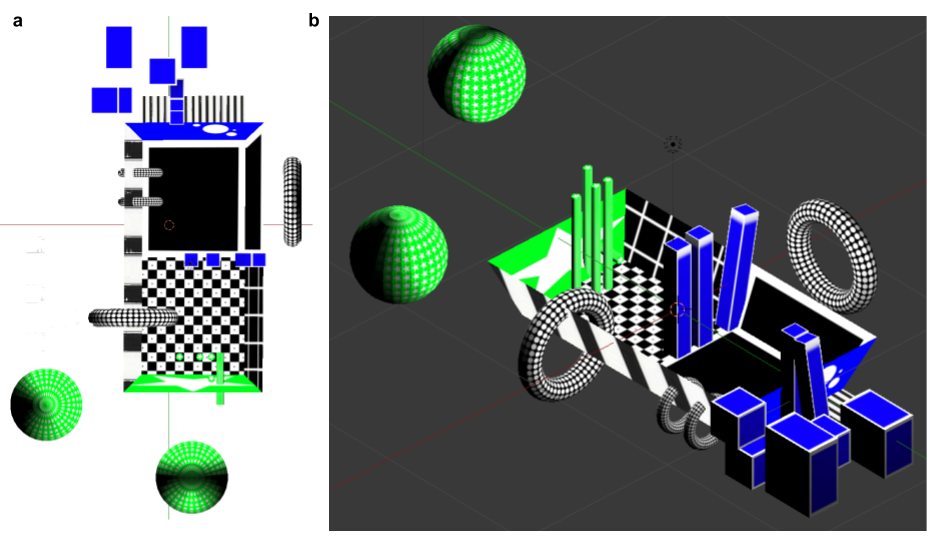
\includegraphics[width=150mm]{figures/F6_virtual_scene.png}}
\caption[Virtual scene]{
Model of the virtual environment for the ratCAVE Virtual Reality setup. (a) Top view of the Virtual environment for vSHIFT and vGAIN experiments (b) Same virtual environment viewed from the Blender modelling software to better see virtual objects and separation in three visually-distinct compartments.
}
\label{fig:F6_virtual_scene}
\end{figure}

The virtual environment consisted of the proximal and distal elements. Distal landmarks were unreachable, they consisted of two green spheres and several blue bricks located at some distance around the arena. The proximal landmarks are represented by landmarks on the arena walls - black and white stripes, black and white plaid, a grey star on a green background, together with distinct visual patterns on the floor - checkerboard pattern, black square pattern, stripes pattern, and virtual objects inside the arena - torus of several sizes, blue and green tall vertical bars. These objects and patterns supported the split of the virtual environment in three distinct “compartments”, which were chosen specifically to induce maximum visual influence on the animal visual perception system and engage more neurons in coding the visual reference frame (see Figure 6). For example, the “stripes” compartment in the vSHIFT -physical experiment is hidden in the original position of the arena, but is available to the animal in the shifted position. At the same time salient green bars on the other end are not reachable, which overall might induce visually-driven cells to more prominently react on the change.

For all shift and gain experiments animals were kept on the light diet (about 90\% of ad libitum weight); animals were randomly foraging for food pellets inside the ratCAVE arena (see methods). Experimental time and movement protocols are described in detail in the following sections.


\section{Introducing mismatch between stable reference frames}
\label{sec:mismath_frames}

The aim of this experimental series is to identify the distribution of a subset of external sensory inputs (visual, tactile or boundary-defined) to the hippocampal place cells and the interaction of these inputs with the internal proprioceptive signals, crucial for path integration. By probing whether the place fields would follow the 3D virtual visual reference frame or the physical boundary-defined arena frame one could split the influence of visual versus tactile (corner- or boundary- related) stimulus and determine how much they are influenced by path integration.


\begin{figure}
\captionsetup{format=plain}
\makebox[\textwidth]{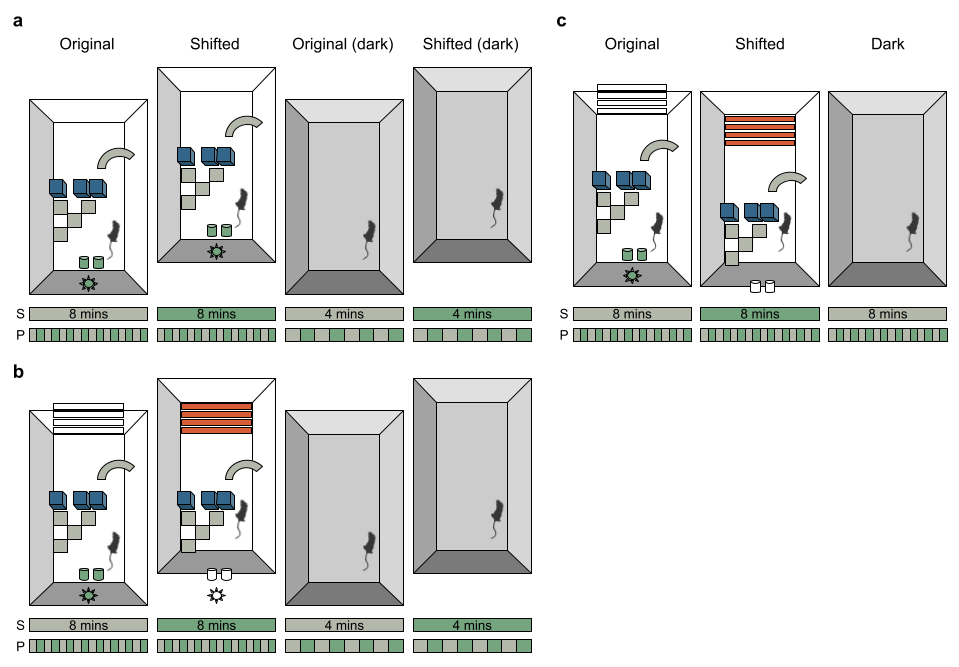
\includegraphics[width=150mm]{figures/F7_vSHIFT.png}}
\caption[vSHIFT]{
Schematic of the concept of the vSHIFT experiment. For all plots: the green/gray bars on the bottom determine the protocol of the arena movement between original and shifted positions. S (single) - a single move, P (periodic) - translation every 30s. (a) vSHIFT - coherent. ratCAVE arena is translated together with the projected virtual objects and visual cues  back and forth along one axis, while the animal is randomly foraging inside. (b) vSHIFT-physical. The arena is periodically translated back and forth while the visual projection (virtual environment) is kept stable in room coordinates. (c) During vSHIFT-visual the arena is kept stable while the visual projection is translated further and back at the same protocol as in (b).
}
\label{fig:F7_vSHIFT}
\end{figure}


\subsection{vSHIFT-coherent - no conflict between reference frames}

To provide an evidence, that the external room cues (e.g. a projector and a mirror) do not play a role in formation of the spatial map, we designed an experiment where the both the arena and the visual scene were moving congruently together in the same time and spatial order as in the previous experiments. As these cues are subtle and hardly seen it is expected that they are ignored by the sensory inputs and do not influence spatial information in the hippocampus as well as the mechanisms of path integration. More precisely, it is expected that none of the units are able to fixate their spatial firing to the room reference frame, and all place fields would move together with the arena and the aligned visual scene. In addition to the experimental evidence of reference frame preference, the resulting distribution of the shift of the place fields could provide statistical metrics (e.g. standard deviation) for these particular conditions (arena length, animal size and behavior), useful for future analysis of other experimental conditions.

In this experiment both the arena and the visual projection were physically moved every 30 seconds in a longitudinal direction for 0.3 meters forth (shifted position, B) and back (original position, A), using the linear actuators located below the arena, like in the physical shift experiment. This action kept visual and border-defined reference frames aligned, while passively moving an animal in allocentric room coordinates (Figure 7a).


\subsection{vSHIFT-physical - conflict between vision and path integration}

In this experiment, a stable visual projection of the 3D virtual environment, containing proximal (virtual bars, torus and pillars) and distal (spheres) landmarks, was projected on the walls of the physical ratCAVE arena. This projection was stable in room coordinates for the whole experiment. To implement a shift, the arena was physically moved every 30 seconds in a longitudinal direction for 0.3 meters forth (shifted position, B) and back (original position, A), using the linear actuators located below the arena. As the projection was stable in room coordinates, it appeared to “shift” inside (relative to) the arena because of the arena move. This introduced a shift between the spatial reference frame, defined by the physical arena boundaries, relative to the visual virtually-defined VR reference frame (see Figure 7b). Neuronal activity was recorded during the whole session, and later only the times when the arena was stationary were analysed. For condition analysis, all periods when arena was in either original (A) or shifted (B) position were integrated to form two separate conditions A and B. For all animals, the session duration was ranging from 12 to 16 minutes, resulting in approx. 6 to 8 minutes of recording in condition A (12-16 arena moves) and 6 to 8 minutes in condition B (12-16 arena moves back).

For some sessions an 8 minutes period of an animal foraging in total darkness was recorded. These result in approx. 4 minutes of recording of the same neuronal units in position A and 4 mins in position B in darkness.

The shift of the arena to position (B) allowed an animal to enter a new virtual area, not available previously in original position (A). This area is marked by horizontal stripes (see Figure 7b, orange). Simultaneously, a virtual area at the end of the virtual scene (with green pillars), was no longer available in position (B) as the physical arena wall prevented an animal from going there. The salient visual landmarks (stripes, pillars) were specifically designed to be present in these areas to engage more place cells to change their activity in two shift conditions.

It is expected that this experiment allows to classify cells by their visual and/or self-motion or boundary-defined selectivity, thus suggesting their possible upstream input types. The behavior of place fields in the need of representing two different reference frames may indicate the way the integration of these pathways is processed in the CA1 pyramidal layer.


\subsection{vSHIFT-visual - alternative way for a conflicting condition}

To probe whether the passive physical movement in space, supported by vestibular signals, is crucial for physical or visual reference frame encoding, it was asked if the shift of the visual scene alone could induce the shift in the encoding of the spatial map. Opposite to the previous physical shift experiment, here the visual projection, containing all distal and proximal virtual landmarks, was moved relative to the stable arena. In original position, the projected virtual scene matched the arena walls similar to the previous experiment, condition A. To introduce a shift, the visual projection was moved every 30 seconds in a longitudinal direction for 0.3 meters forth and back with the same timing, as it would take the physical arena to move. As the physical arena was stationary during the whole experiment, this move introduced a shift between the spatial reference frame, defined by the stationary physical arena boundaries, relative to the changing visual reference frame, with the exception that the animal was not physically moved in room coordinates and the vestibular input pathways were not stimulated (see Figure 7c).

This experimental condition is similar to the physical shift condition with the difference of actual physical move of the arena together with an animal in space or not. As the physical move engages vestibular inputs, this might influence the encoding of one or another reference frame in the hippocampus and might be interesting for a separate research.


\section{Introducing mismatch between vision and proprioception}
\label{sec:mismatch_gain}

The series of experiments targeted to investigate effects on the hippocampal CA1 activity when there is either an instant or spontaneously induced mismatch between visual landmark-defined information and the self-motion, path integration defined information.

\subsection{vGAIN - shift via introducing a gain mismatch between visual flow and proprioception}

Another way of studying the preference for visual versus boundary-defined reference frames for spatial navigation is to introduce a gain mismatch between actual animal movement and the visual flow. Using the VR system, this can be implemented as essentially letting the animal move for a certain distance while moving the visual scene for the same distance multiplied by a coefficient.

To keep all the series of experiments compliant and comparable, we introduced the linear longitudinal gain of the visual flow of 1.2 and 1.5 between the virtual scene and the animal physical translation in a series of 3 stages: original no gain condition, gain condition (when an animal can access extended environment in VR coordinates) and again the no gain condition, when the virtual scene is shifted relative to the arena reference frame (see Figure 8a). Intuitively this experiment is similar to the physical or visual shift experiments (above), with the difference that the shift is performed with the transition via the gain period, when there is a mismatch between the animal longitudinal translation in physical and virtual coordinates.

Each period consisted of 6 minutes recording in every condition with 1 minute between periods, when the gain was linearly increased or decreased. This smooth increase of the gain was required to avoid instant change of the animal position in virtual coordinates and, as a consequence, potential remapping. For some sessions the dark period of 6 minutes was recorded. Recording cell activity in darkness can help in analysis and definition of cells, dependent on visual inputs and their firing behavior after the visual input is cut.

\begin{figure}
\captionsetup{format=plain}
\makebox[\textwidth]{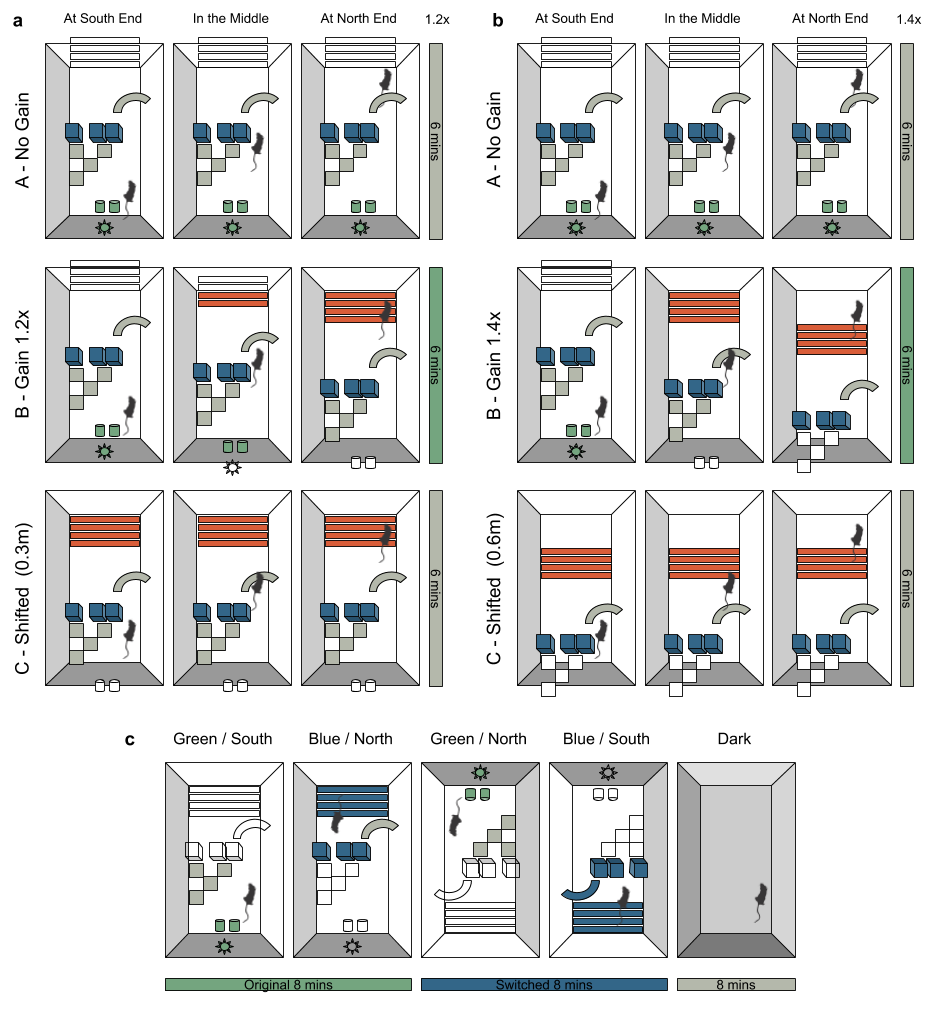
\includegraphics[width=150mm]{figures/F8_vGAIN.png}}
\caption[vGAIN]{
(a) Schematic representation of the vGAIN experiment. Experimental session has 4 periods of original position condition when the animal learns the environment (top row), followed by a gain condition with the extended visual environment fit inside the same physical environment (middle row), and a shifted position condition, where there is no gain but the visual projection is shifted 0.3m relative to the original condition (bottom row). Some sessions followed by a navigation dark (4th period, not shown). Note the visuo-idiothetic spatial conflict between original (A) and gain (B) conditions depends on the position inside the arena (middle row, the conflict is largest at the north of the arena, while there is no conflict on the south of the arena). (b) The same protocol for the vGAIN 1.4x. The difference is the amount of instant (middle row) and resulting (bottom row) conflict ranging from 0 to 0.6m. (c) Schematic representation of the vTELEPORT experiment. Animals learn the environment where the green room is located on the south, and the blue room on the north. Note the projection for only one room where the animal currently is, is active at the same time (left two columns). After an exploration period, green and blue rooms are switched (green room goes north) bringing the conflict between visual cues and path integrator (middle columns). The main conditions are followed by a period of foraging in the dark.
}
\label{fig:F8_vGAIN}
\end{figure}


\subsection{Teleport experiment}

Place cells build spatial maps based on coherent sensory and self-motion-based representations. According to the accumulating evidence (\cite{Gothard1996}, \cite{Samsonovich1997}, \cite{Derdikman2009}) these maps are discrete for distinct environments, associated with unique experiences. Inconsistency between the actual sensory inputs and the recent position history, defined by self-motion and path integration, may introduce a specific type of remapping of the active place representation, referring to one or another discrete spatial map or having a mixture of components (\cite{Jezek2011}).

To study these effects on the level of hippocampal place cells, I designed a virtual teleport experiment. Using the freely-moving virtual reality setup, I designed an environment containing two visually distinct rooms of the same size, that fit the physical VR arena (rooms A and B). While an animal explores room A, the room B was not rendered, so only one room was visually available at a time. Crossing the midline of the arena allowed an animal to move between the rooms. Each room had a hidden circular spot, defined by the proximal visual cues, where an animal could trigger a reward if it stayed within the spot for more than 2 seconds. The rewards were continuously altered between rooms A and B to enforce an animal to navigate between rooms. After the initial learning of the environment for 8 minutes, rooms were switched at the earliest midline crossing, such that it appeared to the animal that it was entering the same room. The switch or the rooms was the central point to investigate whether the mismatch between the previous trajectory (path integration) and a newly imposed visual sensory cues would result in a map substitution or any other type of change in the corresponding place field representation (see Figure 8c).

Due to the time limitations only behavior, but not physiology was recorded with two animals. Behavior recordings demonstrate the ability of animals to learn the reward locations before the switch, as well as quick adaptation to the new orientation of the virtual environment after the room switch (see Figure 8c). This shows the significance of the visual-based virtual representation in original and switched versions and its very probable impact on the spatial map in the brain. However how this teleportation affects the place field maps remains to be investigated.


\section{Comparison of hippocampal spatial activity between ball- and freely-moving VR systems}
\label{sec:comparison_ball_vr}

Previous research on the influence of sensory conditions on the hippocampal place code shows that inactivation of the vestibular system, which severely disrupts the head-direction system, was able to disrupt spatial maps in the hippocampus (\cite{Stackman2002}). While conventional ball-virtual reality systems impose behavioral restrictions such as head- or body fixation they distort parts of the vestibular and proprioceptive inputs, which may result in deformation effects on place cell maps. Understanding the levels of these distortions might be crucial to understand the contribution of self-motion cues to the expression of place fields. The presence of both types of virtual reality setups (ball-VR and ratCAVE VR, see methods and also \cite{Thurley2014}) on-site provided an opportunity to design experiments that compare neuronal activity involved in navigation between the setups, even in the same animal. By recording simple random foraging in the same virtual environment in body-fixed and freely-moving conditions, one could compare neuronal activation patterns, detect differences in place field firing and ultimately better understand the contribution of the vestibular inputs and physical boundaries on the hippocampal place map.

\begin{figure}
\captionsetup{format=plain}
\makebox[\textwidth]{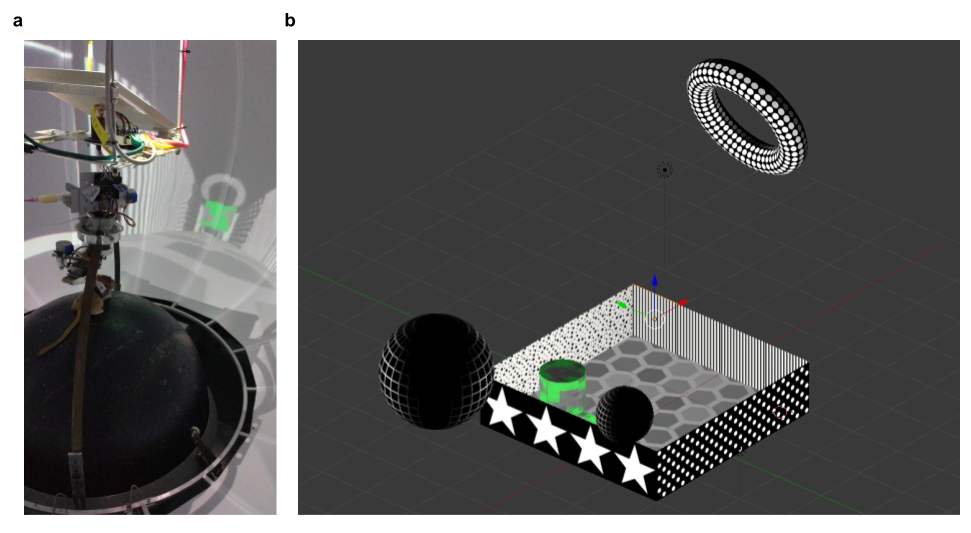
\includegraphics[width=150mm]{figures/F9_ball_VR.png}}
\caption[ball VR]{
Body-fixed virtual reality system. (a) A photo providing an overview of the setup with an animal inside. Animal is held in a harness fixed to the commutator that allows for a 360 degrees rotation. Running on a ball treadmill implements movement in the virtual environment, projected on the screen around the animal. (b) Schematic of the 2D virtual environment used in the beacon navigation task.
}
\label{fig:F9_ball_VR}
\end{figure}

To implement this experiment, I adopted the rendering engine and wrote experimental control software that enables the rendering of the same virtual environment in both VR setups (see methods). I designed a simple 2D environment and a beacon foraging task where gerbils need to navigate to a green beacon, which was changing its position every trial, to get a reward (20mg sucrose pellets in the ratCAVE setup, a 0.1ml dose of sweet milk in the ball setup).

While a freely-moving situation does not require any specific pre-conditioning, ball-virtual reality requires extensive handling and animal adaptation to being restricted by a harness. In gerbils, this restriction does not always lead to a successful animal adaptation and, empirically, depends on animal age, personal character and status in the cohort. As a result, many animals do not feel comfortable in the harness or even build aversion to both harness and setup. Practically this results in either animal freezing while being in the setup on the styrofoam ball, or a periodic running in a single direction, supposedly ignoring the visual projection, with an appearance aimed at escaping. Overall, such animal behavior even after extensive training and adaptation (4-5 weeks) does not always allow for navigation in a 360 virtual 2D environment. Actual training results show on average one out of four animals capable of adapting to the harness and setup, learning the 360 rotation, reward system and 2D navigation for a salient green beacon (not shown in this work). This imposes restrictions on the timing for the surgery: first - one has to train animals to select the right candidate, and second - it increases the risk of an overall wasted time, in case the surgery or recovery does not go well. Ultimately there was a decision to freeze this type of experiment until there is a better and more stable solution for animal training and harness adaptation.
